\chapter{Perancangan}
Berdasarkan analisis yang telah dilakukan, terdapat beberapa hal yang perlu dirancang untuk pembangunan perangkat lunak naive bayes berbasis \textit{hadoop mapreduce}. Pada bab ini akan dijelaskan perancangan yang diperlukan untuk membangun perangkat lunak yaitu perancang-
an antarmuka, diagram kelas rinci, serta rincian metode.
			
\section{Perancangan Antarmuka}

Perangkat lunak \textit{naive bayes classification} memiliki 6 buah tampilan untuk yang tidak berbasis \textit{MapReduce}, yaitu: (1) \textit{Dashboard} (2) \textit{Input Set Manager} (3) \textit{Renew Model Manager} (4) \textit{Testing Manager} (5) \textit{Classification Manager} (6) \textit{Error Rate Dashboard}. Untuk program yang berbasis \textit{MapReduce} tidak akan memiliki antarmuka yang khusus, karena program hanya perlu dijalankan dengan menggunakan CLI (\textit{command line interface}). Berikut adalah penjelasan dan gambar dari tiap antarmuka yang dirancang:

\subsection{\textit{Dashboard}}

\begin{figure}[H]
	\centering
	\includegraphics[scale=0.45]{Mockup/mockup_dashboard_0}
	\caption[input-set-gui-1]{Dashboard}
	\label{fig:input-set-gui-1}
\end{figure}
\textit{Dashboard} dibuat untuk memudahkan user dalam memonitor model NBC yang telah dimasukkan ke dalam perangkat lunak yang dibangun. Berikut penjelasan lebih lanjut mengenai tiap komponen pada rancangan \textit{dashboard} yang dibuat:
\begin{enumerate}
	\item Berisi nama - nama atribut kelas dan total frekeunsi kemunculannya tiap nilai.
	\item Berisi nama - nama atribut prediktor dan frekuensi kemunculannya untuk prediktor bertipe diskrit dan \textit{mean} \verb|&| \textit{sigma} untuk yang bertipe numerik.
	\item \textit{Bayesian model} merupakan model dari NBC yang akan digunakan untuk testing dan klasifikasi. Model ini merupakan model yang langsung di-import dari hasil training di dalam HDFS.
\end{enumerate}

\subsection{\textit{Input Set Manager}}
\begin{figure}[H]
	\centering
	\includegraphics[scale=0.4]{Mockup/input-set-gui-1}
	\caption[\textit{Input Set Manager}]{\textit{Input Set Manager}}
	\label{fig:Input Set Manager}
\end{figure}
\textit{Input Set Manager} dibuat untuk memudahkan user melakukan input data ke dalam HDFS menggunakan perangkat lunak yang dibuat. Berikut penjelasan lebih lanjut mengenai tiap komponen pada rancangan \textit{Input Set Manager} yang dibuat:
\begin{enumerate}
	\item User dapat memilih tipe model input yang sudah ada dalam HDFS.
	\item Jika ingin membuat tipe model input baru pada HDFS, maka user perlu mengisi kolom ini dan mengisi nama model yang diinginkan.
	\item User dapat memilih file input yang akan dikirimkan ke dalam HDFS. User dapat memilih > 1 file sekaligus.
	\item User dapat memilih file info mengenai file input, yang dikirimkan ke dalam HDFS.
	\item User dapat memilih presentase pembagian data antara data \textit{training} dan data \textit{testing} dari keseluruhan data input yang akan dimasukkan ke dalam HDFS.
	\item Setelah memillih file info, user dapat memilih atribut mana saja yang akan digunakan untuk training. User juga dapat memilih tipe(diskrit/numerik) dari atribut tersebut beserta jenisnya (kelas/prediktor).
\end{enumerate}

\subsection{\textit{Renew Model Manager}}
\begin{figure}[H]
	\centering
	\includegraphics[scale=0.45]{Mockup/mockup_renewmodel_manager}
	\caption[\textit{Renew Model Manager}]{\textit{Renew Model Manager}}
	\label{fig:Renew Model Manager}
\end{figure}
\textit{Renew Model Manager} dibuat agar user selalu bisa memperbaharui model NBC pada perangkat lunak yang dibikin.
\begin{enumerate}
	\item User dapat memilih file model NBC hasil dari training dari sistem penyimpanan \textit{local}.
	\item User dapat memilih file model NBC hasil dari training langsung dari HDFS.
\end{enumerate}

\subsection{\textit{Testing Manager}}
\begin{figure}[H]
	\centering
	\includegraphics[scale=0.45]{Mockup/mockup_testing_manager}
	\caption[\textit{Testing Manager}]{\textit{Testing Manager}}
	\label{fig:Testing Manager}
\textit{Testing Manager} dibuat untuk melakukan testing pada model NBC yang sudah di-import ke dalam program sebelumnya.
\end{figure}
\begin{enumerate}
	\item User dapat memilih file input dan file info dari penyimpanan \textit{local} milik user.
	\item User dapat memilih file testing yang sudah ada di dalam HDFS dengan memilih model input direktori pada HDFS.
\end{enumerate}

\subsection{\textit{Classification Manager}}
\begin{figure}[H]
	\centering
	\includegraphics[scale=0.45]{Mockup/mockup_classification_manager}
	\caption[\textit{Classification Manager}]{\textit{Classification Manager}}
	\label{fig:Classification Manager}
\end{figure}
\textit{Classification Manager} dapat digunakan untuk mengklasifikasi satu record input/kasus yang secara langsung diisi sendiri oleh user yang menggunakannya terhadap model NBC yang sudah ada pada perangkat lunak sebelumnya.
\begin{enumerate}
	\item User memilih nilai prediktor untuk kasus baru (prediktor dapat berupa dropdown untuk yang bertipe diskrit dan \textit{number} untuk yang bertipe numerik)
	\item User dapat memilih kelas yang menjadi prediksi sebelumnya dari user untuk diperiksa kebenarannya jika menggunakan program setelah diklasifikasikan menggunakan model NBC yang sudah ada.
	\item Hasil dari klasifikasi yang telah dijalankan.
\end{enumerate}

\subsection{\textit{Error Rate Dashboard}}
\begin{figure}[H]
	\centering
	\includegraphics[scale=0.45]{Mockup/mockup_errorrate}
	\caption[\textit{Error Rate Dashboard}]{\textit{Error Rate Dashboard}}
	\label{fig:Error Rate Dashboard}
\end{figure}
\textit{Error Rate Dashboard} dibuat untuk memonitor hasil \textit{error rate} yang sudah dihitung setelah menjalani proses testing. 
\begin{enumerate}
	\item \textit{Confusion matrix} untuk setiap atribut kelas.
	\item Error rate yang akan dihasilkan setelah melakukan klasifikasi meliputi: (1)$Accuracy$; (2)$Precision$; (3)$Recall$; (4)$F-Measure$.
\end{enumerate}



\section{Diagram Kelas Lengkap dan Design Pattern}
Berikut adalah penjelasan dari kelas - kelas pada keempat modul yang dibuat beserta penjelasan setiap atribut dan operasi yang dimiliki oleh kelas - kelas tersebut.

\subsection{Diagram Kelas Modul \textit{Train Naive Bayes M-R Based}}
Pada diagram kelas ini terdapat terdapat 2 \textit{package} utama yang akan menjadi inti dari modul ini, salah satunya merupakan \textit{package} yang dimiliki oleh \textit{library} dari \textit{hadoop client} untuk dapat menjalankan proses \textit{mapreduce}. Berikut adalah gambar dari \textit{package - package} tersebut:
\begin{figure}[H]
	\centering
	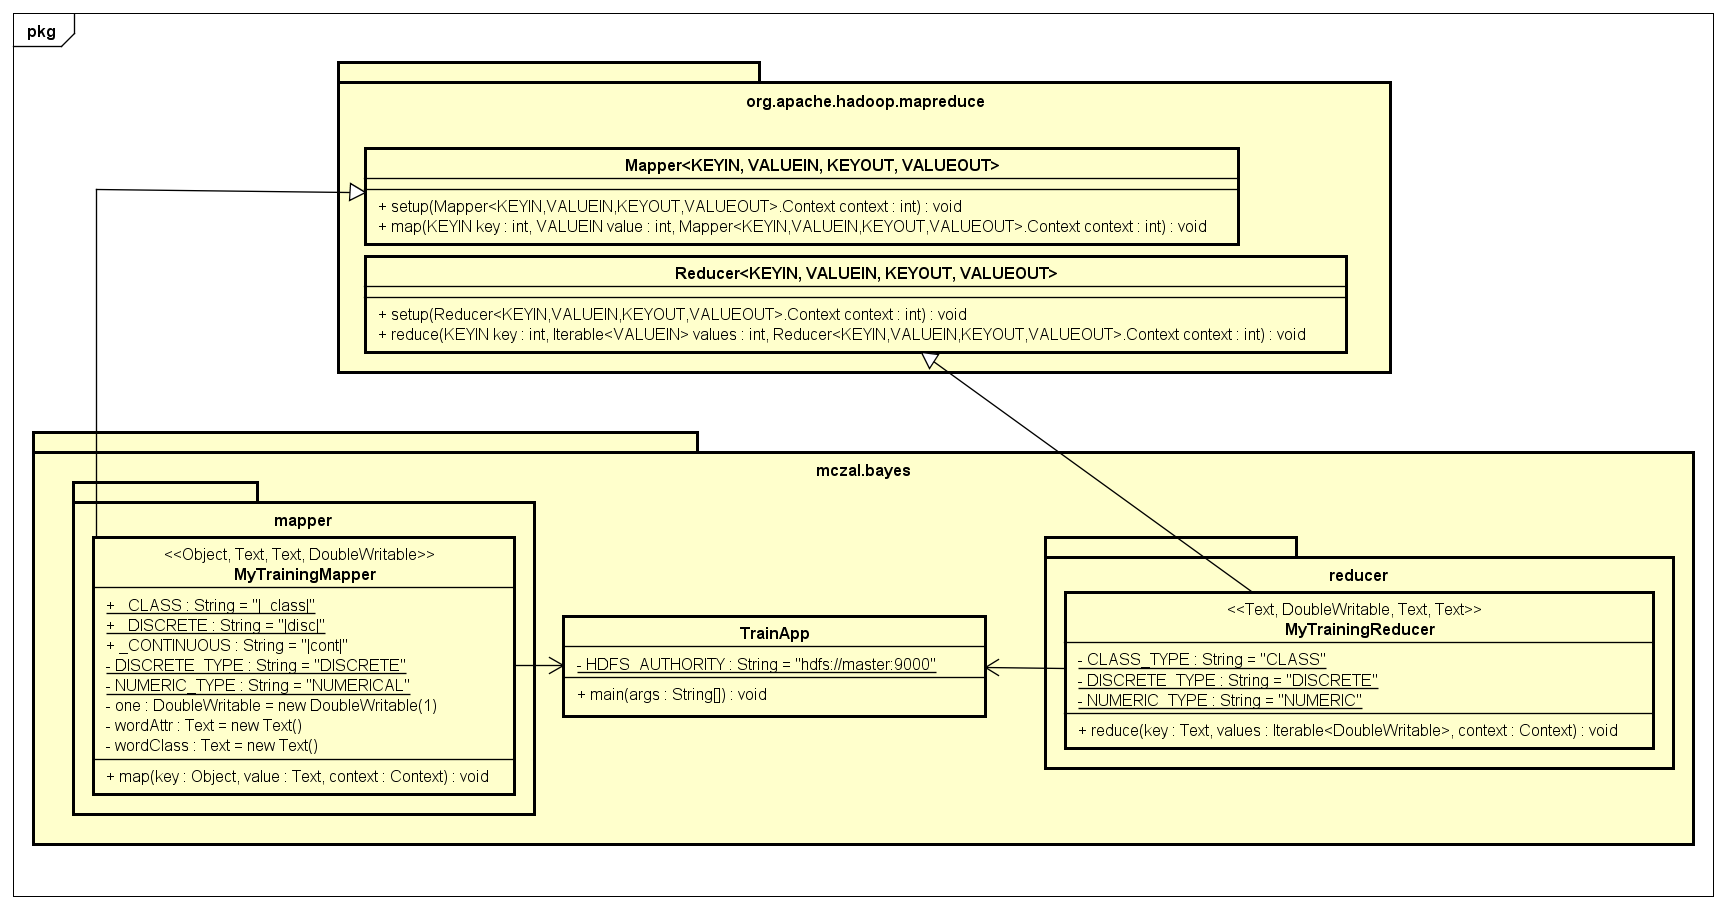
\includegraphics[scale=0.6]{ClassDiagramLengkap/CD_Train_MR}
	\caption[Diagram Kelas \textit{Train Naive Bayes M-R Based}]{\textit{Diagram Kelas Train Naive Bayes M-R Based}}
	\label{fig:Diagram Kelas Modul Kelola Input}
\end{figure}

\paragraph{\textit{Package} $org.apache.hadoop.mapreduce$}
Dalam \textit{package} ini terdapat 2 kelas utama yang akan menjadi kelas \textit{parent} dari kelas \textit{reducer} dan \textit{mapper} yang di-implementasikan.
\begin{enumerate}
	\item{Kelas \textit{Mapper}}\\
	Kelas ini memiliki 4 buah \textit{generic types}\footnote{A generic type is a generic class or interface that is parameterized over types \cite{GenericTypeJavaOracle}} yang perlu di-implementasikan pada kelas yang mengimplementasi method ini. Parameter \textit{generic types} tersebut antara lain adalah:
	\begin{itemize}
		\item{\textit{KEYIN}}\\
		Kelas ini merupakan tipe kelas yang akan menjadi \textit{key} masukan pada proses Map untuk program \textit{Mapreduce} yang dibuat.		
		\item{\textit{VALUEIN}}\\
		Merupakan tipe kelas yang akan menjadi \textit{value} dari masukan pada proses Map untuk program \textit{Mapreduce} yang dibuat.
		\item{\textit{KEYOUT}}\\
		Merupakan tipe kelas yang akan menjadi \textit{key} keluaran pada proses Map untuk program \textit{Mapreduce} yang dibuat.
		\item{\textit{VALUEOUT}}\\
		Merupakan tipe kelas yang akan menjadi \textit{value} keluaran pada proses Map untuk program \textit{Mapreduce} yang dibuat.
	\end{itemize}
	
	\item{Kelas \textit{Reducer}}\\
	Kelas ini memiliki 4 buah \textit{generic types} yang perlu di-implementasikan pada kelas yang mengimplementasi method ini. Parameter \textit{generic types} tersebut antara lain adalah:
	\begin{itemize}
		\item{\textit{KEYIN}}\\
		Kelas ini merupakan tipe kelas yang akan menjadi \textit{key} masukan pada proses \textit{Reduce} untuk program \textit{Mapreduce} yang dibuat.		
		\item{\textit{VALUEIN}}\\
		Merupakan tipe kelas yang akan menjadi \textit{value} dari masukan pada proses \textit{Reduce} untuk program \textit{Mapreduce} yang dibuat.
		\item{\textit{KEYOUT}}\\
		Merupakan tipe kelas yang akan menjadi \textit{key} keluaran pada proses \textit{Reduce} untuk program \textit{Mapreduce} yang dibuat.
		\item{\textit{VALUEOUT}}\\
		Merupakan tipe kelas yang akan menjadi \textit{value} keluaran pada proses \textit{Reduce} untuk program \textit{Mapreduce} yang dibuat.
	\end{itemize}
\end{enumerate}

\paragraph{\textit{Package} $mczal.bayes$}
Dalam \textit{package} ini terdapat beberapa \textit{package} lagi dan kelas - kelas yang akan dijadikan implementasi dari kelas \textit{Mapper} dan \textit{Reducer} pada package \textit{org.apache.hadoop.mapreduce} untuk proses \textit{MapReduce}.
\begin{enumerate}
	\item{Kelas \textit{TrainApp}}\\
	Kelas ini merupakan kelas utama(\textit{main class}) yang akan dijalankan pertama kali program ini dieksekusi. Kelas ini memiliki 1 atribut \textit{static} dan 1 method \textit{main}.
	\begin{enumerate}
		\item Atribut \verb|HDFS_AUTHORITY| \\
		Atribut ini bertipe \textit{String} dan memiliki \textit{modifier} \textit{static} dan \textit{final} agar nilainya tidak dapat diubah - ubah. Inisialisasi pertama dari atribut ini adalah: \verb|"hdfs://master:9000"|. \verb|"hdfs://master:9000"| merupakan url dari node master yang digunakan untuk dapat berkomunikasi dengan node master pada lingkungan \textit{hadoop}. Atribut ini digunakan untuk \textit{request} operasi baca file \textit{meta.info} pada HDFS.
		
		\item Operasi \verb|main|\\
		Operasi ini akan menjadi operasi pertama yang dijalankan ketika melakukan eksekusi program mapreduce pada modul ini. Operasi ini akan men-\textit{set} kelas \textit{mapper} dan kelas \textit{reducer} yang akan digunakan serta variabel - variabel yang perlu dikirimkan kepada tiap node yang dibutuhkan oleh mereka.
	\end{enumerate}

	\item{Kelas \textit{MyTrainingMapper}}\\
	Kelas ini merupakan kelas turunan dari kelas \textit{Mapper} yang ada pada package \verb|org.apache.hadoop.mapreduce|. \textit{Generic type} kelas parent dari kelas ini adalah:
	\begin{enumerate}
		\item{Object} merupakan tipe \textit{key} masukan dari proses \textit{map}.
		\item{Text} merupakan tipe \textit{key} masukan dari proses \textit{map}. Karena, data masukan akan berupa \textit{string}.
		\item{Text} merupakan tipe \textit{key} keluaran dari proses \textit{map}. Karena, \textit{key} pada hasil dari fase \textit{map} akan mengeluarkan data yang bertipe \textit{string}.
		\item{DoubleWritable} merupakan tipe \textit{value} keluaran dari proses \textit{map}. Karena, \textit{value} keluaran pada proses \textit{map} akan berisi jumlah frekuensi atau nilai dari atribut prediktor-numerik yang bertipe numerik.
	\end{enumerate}
	Kelas ini memiliki 8 atribut. Diantaranya adalah:
	\begin{enumerate}
		\item \verb|_CLASS| merupakan atribut bertipe \textit{string} yang memiliki \textit{modifier} \textit{static} dan \textit{final}. Atribut ini memiliki nilai inisialisasi awal = $"|$\verb|_|$class|"$ yang akan digunakan untuk membedakan bahwa data keluaran yang memiliki string berisi $"|$\verb|_|$class|"$ merupakan data keluaran yang akan digunakan untuk menghitung jumlah frekuensi dari kemunculan atribut bertipe kelas.
		\item \verb|_DISCRETE| merupakan atribut bertipe \textit{string} yang memiliki \textit{modifier} \textit{static} dan \textit{final}. Atribut ini memiliki nilai inisialisasi awal = $"|disc|"$ yang akan digunakan untuk membedakan bahwa data keluaran yang memiliki string berisi $"|disc|"$ merupakan data keluaran yang akan digunakan untuk menghitung jumlah frekuensi dari kemunculan atribut prediktor bertipe diskrit berdasarkan atribut kelas tertentu.
		\item \verb|_CONTINUOUS| merupakan atribut bertipe \textit{string} yang memiliki \textit{modifier} \textit{static} dan \textit{final}. Atribut ini memiliki nilai inisialisasi awal = $"|cont|"$ yang akan digunakan untuk membedakan bahwa data keluaran yang memiliki string berisi $"|cont|"$ merupakan data keluaran yang akan digunakan untuk mencatat nilai dari atribut numerik berdasarkan atribut kelas tertentu.
		\item \verb|DISCRETE_TYPE| merupakan atribut bertipe \textit{string} yang memiliki \textit{modifier} \textit{static} dan \textit{final}. Atribut ini memiliki nilai inisialisasi awal = $"DISCRETE"$ yang akan digunakan untuk membedakan bahwa data input setelah displit dengan regex ',' pada indeks tertentu memiliki info bertipe diskrit.
		\item \verb|NUMERIC_TYPE| merupakan atribut bertipe \textit{string} yang memiliki \textit{modifier} \textit{static} dan \textit{final}. Atribut ini memiliki nilai inisialisasi awal = $"NUMERICAL"$ yang akan digunakan untuk membedakan bahwa data input setelah displit dengan regex ',' pada indeks tertentu memiliki info bertipe numerik.
		\item \verb|one| merupakan atribut bertipe \textit{DoubleWritable} yang memiliki \textit{modifier} \textit{static}. Atribut ini memiliki nilai inisialisasi awal = integer bernilai 1 yang akan digunakan untuk mencatat tiap kemunculan atribut prediktor terhadap atribut kelas tertentu yang sedang diperiksa dengan jumlah kemunculan sebanyak 1.
		\item \verb|wordAttr| merupakan atribut bertipe \textit{Text} yang memiliki \textit{modifier} \textit{static}. Atribut ini akan digunakan untuk mencatat tiap atribut prediktor yang akan ditulis menjadi \textit{output key} untuk perhitungan probabilitas posterior dari atribut tertentu pada atribut kelas tertentu.
		\item \verb|wordClass| merupakan atribut bertipe \textit{Text} yang memiliki \textit{modifier} \textit{static}. Atribut ini akan digunakan untuk mencatat tiap kemunculan atribut kelas tertentu dan akan ditulis menjadi \textit{output key} untuk perhitungan frekuensi atribut kelas.
	\end{enumerate}
	Kelas ini memiliki 1 buah operasi. Operasi tersebut adalah operasi \textit{map(key : Object, value : Text, context : Context) : void} yang akan melakukan operasi pada fase map untuk proses training pada modul ini. Seperti yang digambarkan pada DFD sebelumnya, proses ini akan melakukan perhitungan jumlah frekuensi kemunculan tiap atribut. Terkecuali untuk atribut prediktor yang bertipe numerik, operasi ini akan mengeluarkan kembali nilai yang dibaca dari input.
	
	\item{Kelas \textit{MyTrainingReducer}}\\
	Kelas ini merupakan kelas turunan dari kelas \textit{Reducer} pada \textit{package org.apache.hadoop.mapreduce}. \textit{Generic type} kelas parent dari kelas ini adalah: 
	\begin{enumerate}
		\item Text merupakan tipe \textit{key} masukan dari proses \textit{reduce} yang dikirim dari proses sebelumnya yaitu proses \textit{map}
		\item DoubleWritable merupakan tipe \textit{value} masukan dari proses \textit{reduce} yang dikriim dari proses sebelumnya yaitu proses \textit{map}.
		\item Text merupakan tipe \textit{key} keluaran dari proses \textit{reduce}. Karena data keluaran berupa model NBC akan memiliki key berisi string.
		\item Text merupakan tipe \textit{value} keluaran dari proses \textit{reduce}. Karena data keluaran berupa model NBC akan memiliki \textit{value} berisi string.
	\end{enumerate}
	Kelas ini memiliki 3 atribut yang memiliki \textit{modifier} \textit{static} dan \textit{final}. Atribut tersebut diantaranya adalah:
	\begin{enumerate}
		\item \verb|CLASS_TYPE| merupakan atribut bertipe string yang memiliki nilai inisialisasi awal = \textit{"CLASS"}. Atribut ini akan digunakan sebagai pembeda pada data keluaran yang merupakan atribut kelas.
				
		\item \verb|DISCRETE_TYPE| merupakan atribut bertipe string yang memiliki nilai inisialisasi awal = \textit{"DISCRETE"}. Atribut ini akan digunakan sebagai pembeda pada data keluaran yang merupakan atribut prediktor bertipe diskrit.

		\item \verb|NUMERIC_TYPE| merupakan atribut bertipe string yang memiliki nilai inisialisasi awal = \textit{"NUMERIC"}. Atribut ini akan digunakan sebagai pembeda pada data keluaran yang merupakan atribut prediktor bertipe numerik.
	\end{enumerate}
	
	Kelas ini memiliki 1 buah operasi. Operasi tersebut adalah operasi \textit{reduce(key : Text, values : Iterable<DoubleWritable>, context : Context) : void} yang akan melakukan operasi pada fase reduce untuk proses training pada modul ini. Seperti yang digambarkan pada DFD sebelumnya, proses ini akan melakukan akumulasi dari tiap perhitungan jumlah frekuensi kemunculan tiap value yang memiliki key yang sama. Terkecuali untuk atribut prediktor yang bertipe numerik, operasi ini akan menghitung nilai rata - rata dari tiap value pada key tersebut dan lalu dilanjutkan menghitung nilai standar deviasi pada probabilitas posterior atribut numerik tersebut.

\begin{algorithm}
\caption{NBC Model algorithm}\label{euclid}
\begin{algorithmic}[1]
\Procedure{Map}{$key,value,context$}\Comment{Map function}
\State $ $\verb|_|$CLASS \gets "|$\verb|_|$class|"$
\State $ $\verb|_|$DISCRETE \gets "|disc|"$
\State $ $\verb|_|$CONTINUOUS \gets "|cont|"$
\State $ one \gets 1$
\State $ NUMERIC$\verb|_|$TYPE \gets "NUMERICAL"$
\State $ DISCRETE$\verb|_|$TYPE \gets "DISCRETE"$

\State $ countColumn \gets getInputColumnCount$
\State $ inputSplit[] \gets value.split(',')$
\If{inputSplit.length != countCols}\Comment{Ignoring missing values}
	\State \Return
\EndIf

\State $classConf \gets getClassInfo$\Comment{get class info from meta.info}
\State $classSplitConf[] \gets classConf.split(";")$

\State $attrConf \gets getAttributeInfo$\Comment{get predictor info from meta.info}
\State $attrSplitConf[] \gets attrConf.split(";")$

\State $checkerClassPrior \gets classSplitConf.length$
%\For $i \gets 0$ \To $attrSplitConf.length$ \Do
\For{$i \gets 0$ \textbf{to} $attrSplitConf.length$}	
	\If{$attrSplitConf[i].split(",")[2].equals(DISCRETE_TYPE)$}
		%\For $j \gets 0$ \To $classSplitConf.length$ \Do
		\For{$j \gets 0$ \textbf{to} $classSplitConf.length$}	
			\State $currKey \gets $\verb|_| $DISCRETE + attrSplitConf[i].split(",")[0]
              + "," + inputSplit[Integer.parseInt(attrSplitConf[i]
              .split(",")[1])]
              + "," + classSplitConf[j].split(",")[0]
              + "," + inputSplit[Integer.parseInt(classSplitConf[j]
              .split(",")[1])];$
          	\State $wordAttr.set(currKey);$
          	\State $context.write(wordAttr, one)$
		\EndFor
	\EndIf
\EndFor

\EndProcedure
\end{algorithmic}
\end{algorithm}
	
\end{enumerate}

\subsection{Diagram Kelas Modul \textit{Testing Naive Bayes M-R Based}}

\subsubsection{Kelas \textit{Main}}
\begin{figure}[H]
	\centering
	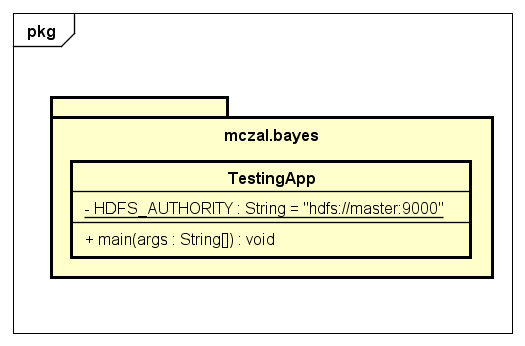
\includegraphics[scale=0.7]{ClassDiagramLengkap/CD_Test_Main}
	\caption[Diagram Kelas Modul \textit{Testing: Main}]{Diagram Kelas Modul \textit{Testing: Main}}
	\label{fig:Diagram Kelas Modul Testing: Main}
\end{figure}

\subsubsection{\textit{Package Base}}
\begin{figure}[H]
	\centering
	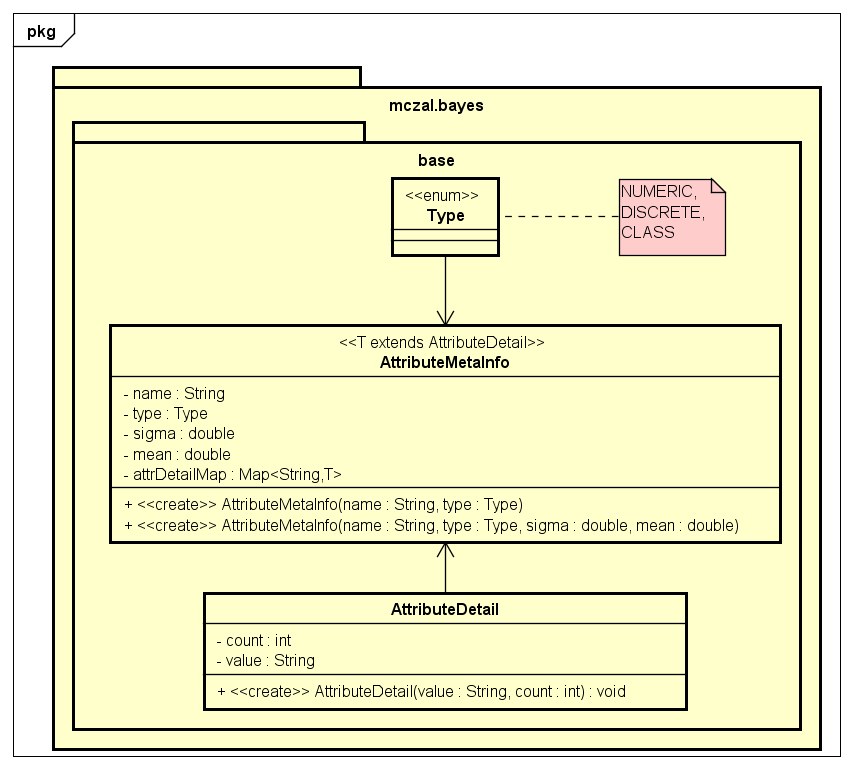
\includegraphics[scale=0.64]{ClassDiagramLengkap/CD_Test_BASE}
	\caption[Diagram Kelas Modul \textit{Testing: Package Base}]{Diagram Kelas Modul \textit{Testing: Package Base}}
	\label{fig:Diagram Kelas Modul Testing: Package Base}
\end{figure}

\subsubsection{\textit{Package Mapper}}
\begin{figure}[H]
	\centering
	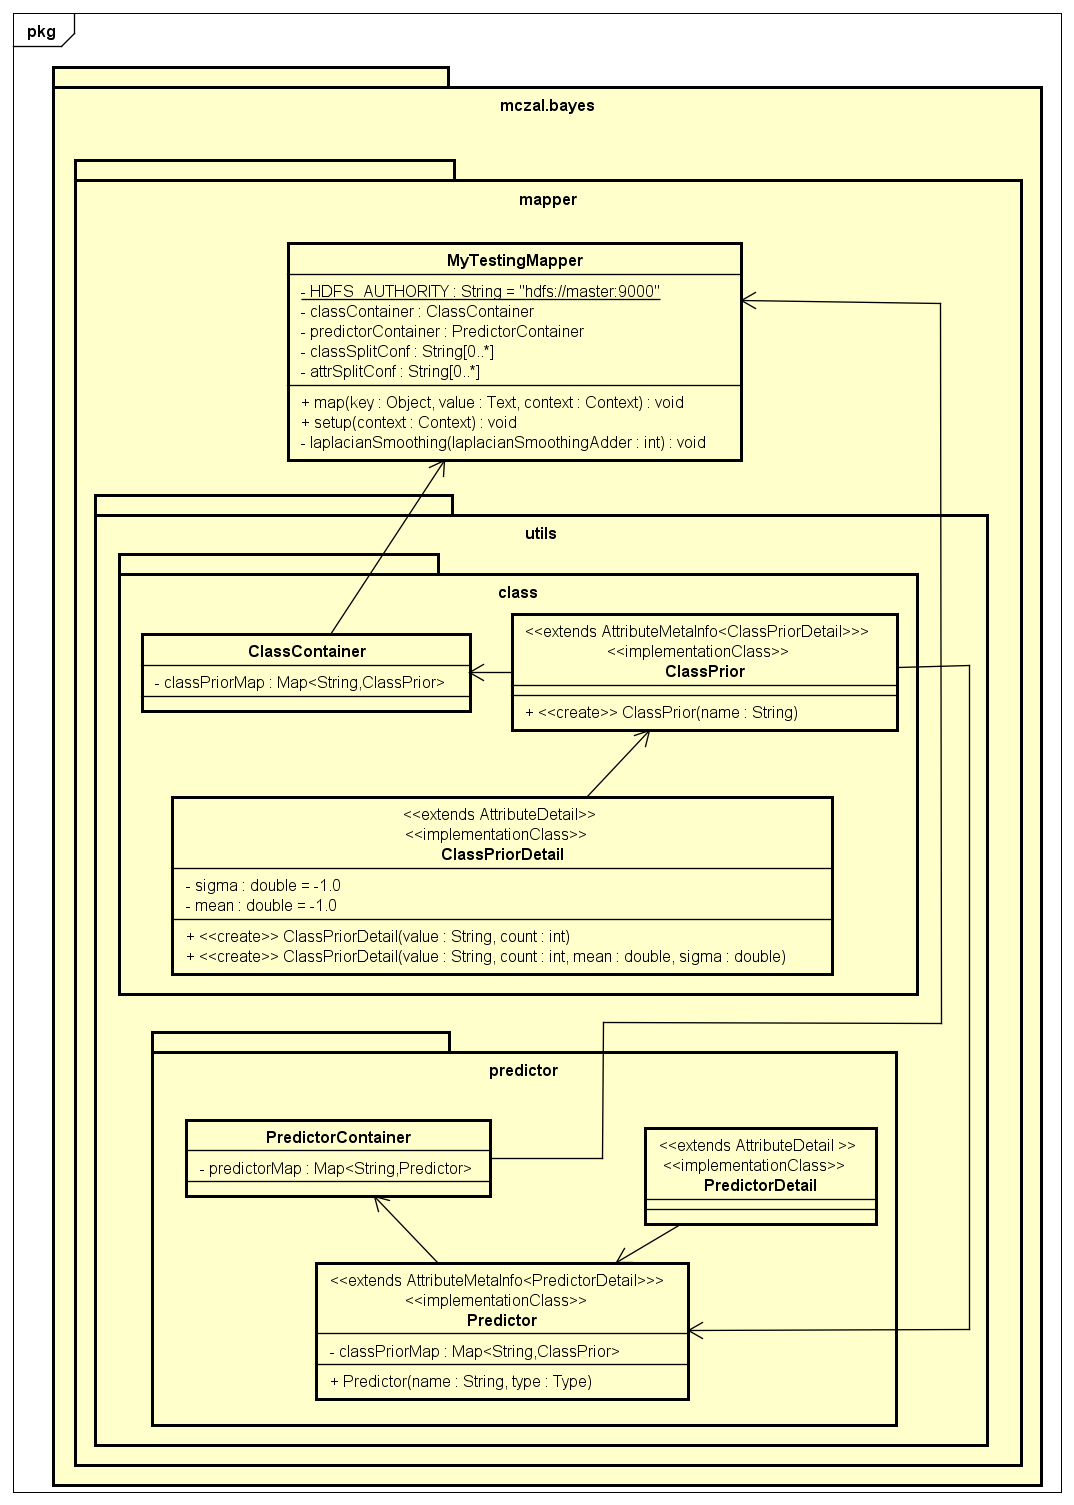
\includegraphics[scale=0.6]{ClassDiagramLengkap/CD_Test_Mapper}
	\caption[Diagram Kelas Modul \textit{Testing: Package Mapper}]{Diagram Kelas Modul \textit{Testing: Package Mapper}}
	\label{fig:Diagram Kelas Modul Testing: Package Mapper}
\end{figure}

\subsubsection{\textit{Package Reducer}}
\begin{figure}[H]
	\centering
	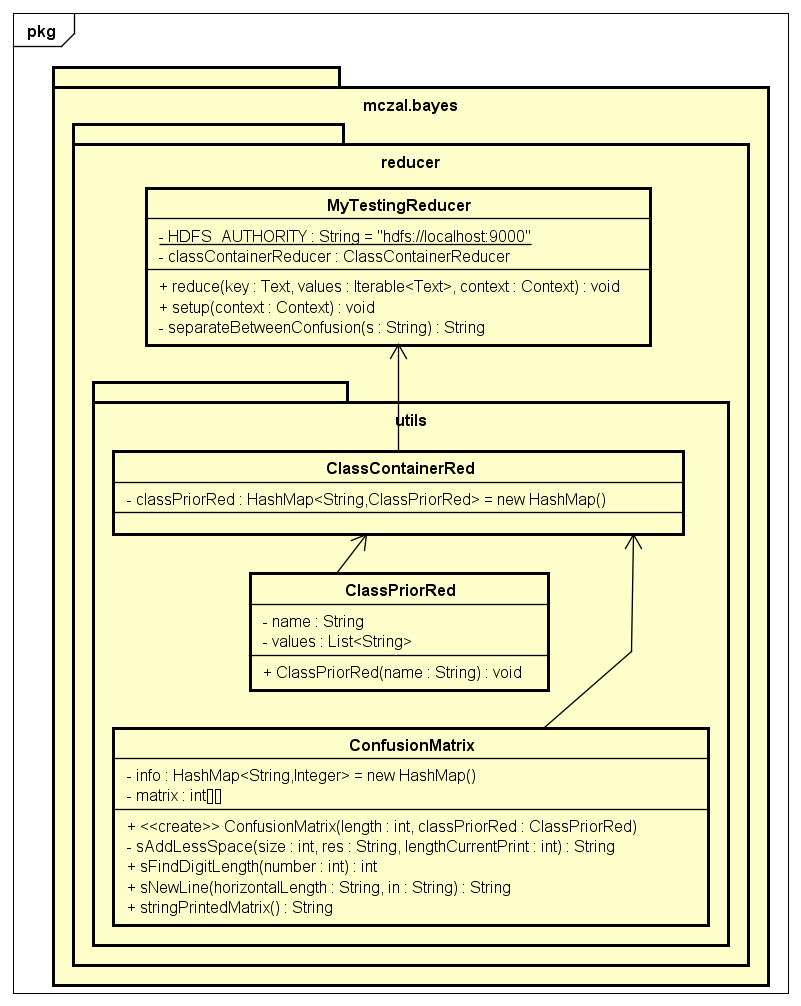
\includegraphics[scale=0.7]{ClassDiagramLengkap/CD_Test_Reducer}
	\caption[Diagram Kelas Modul \textit{Testing: Package Reducer}]{Diagram Kelas Modul \textit{Testing: Package Reducer}}
	\label{fig:Diagram Kelas Modul Testing: Package Reducer}
\end{figure}


\subsection{\textit{Design Pattern} Modul Kelola Input dan Modul Klasifikasi \textit{Naive Bayes}}
\begin{figure}[H]
	\centering
	\includegraphics[scale=0.7]{ClassDiagramLengkap/springmvc}
	\caption[Design Pattern Modul Klasifikasi]{Design Pattern Modul Klasifikasi}
	\label{fig:Design Pattern Modul Klasifikasi}
\end{figure}


\subsection{Diagram Kelas Modul Kelola Input}

\begin{figure}[H]
	\centering
	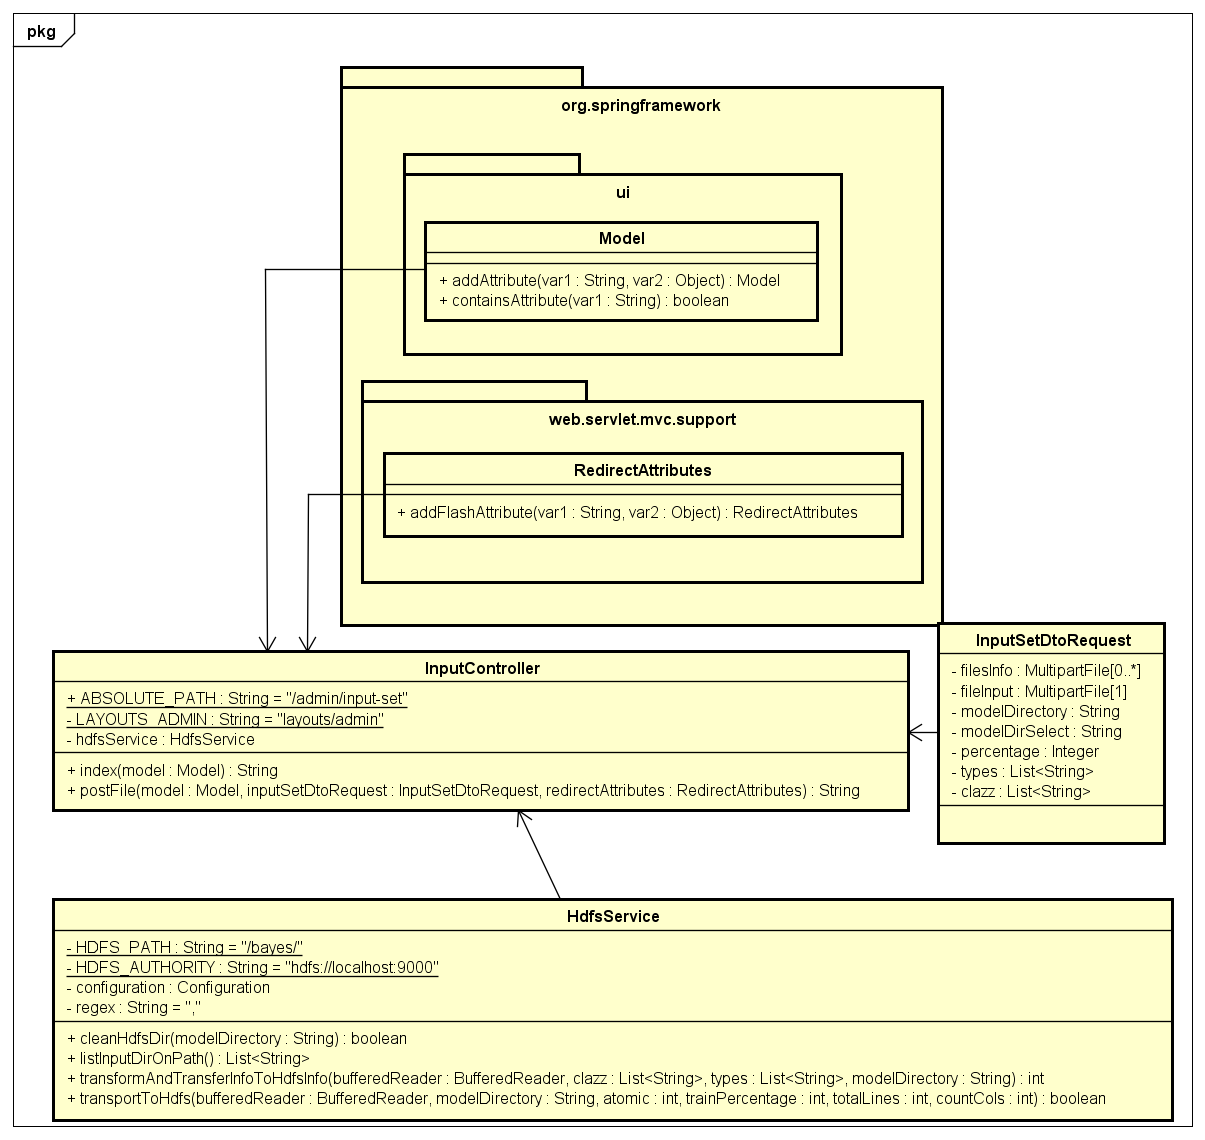
\includegraphics[scale=0.85]{ClassDiagramLengkap/CD_Input}
	\caption[Diagram Kelas Modul Kelola Input]{Diagram Kelas Modul Kelola Input}
	\label{fig:Diagram Kelas Modul Kelola Input}
\end{figure}

\subsection{Diagram Kelas Modul Klasifikasi \textit{Naive Bayes}}

\subsubsection{\textit{Controller}}
\begin{figure}[H]
	\centering
	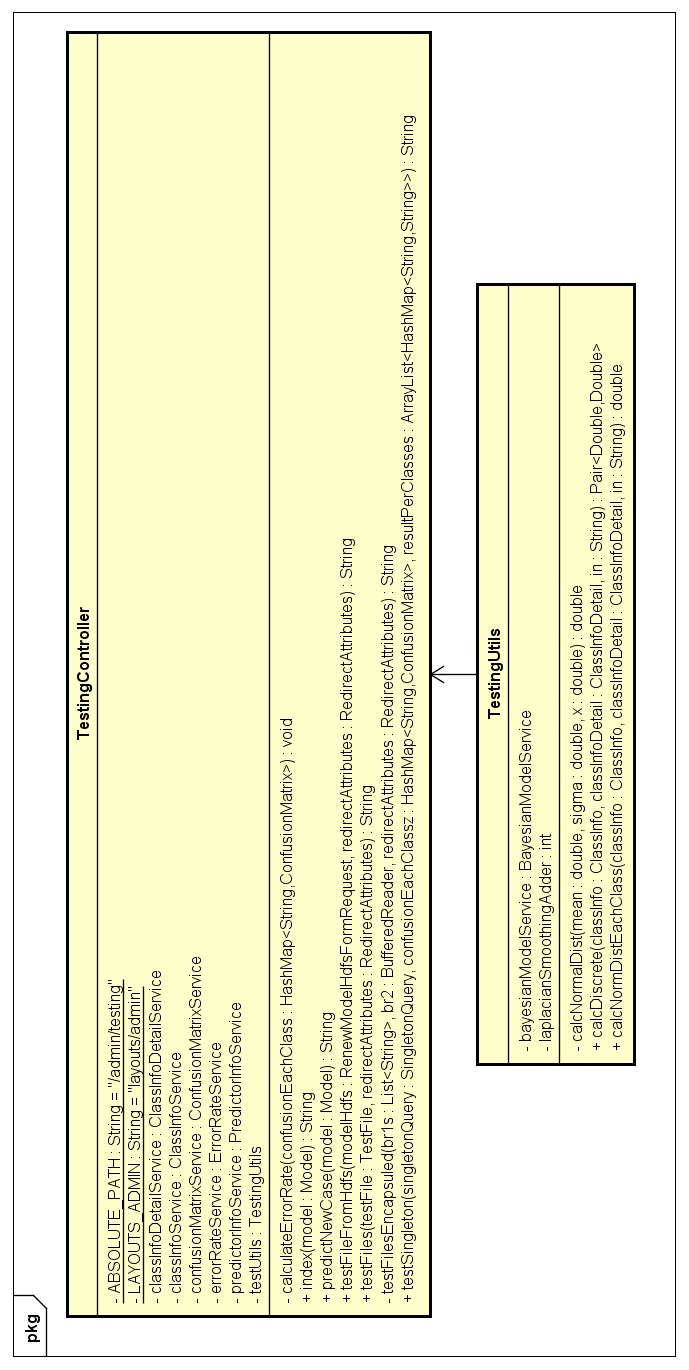
\includegraphics[scale=0.6]{ClassDiagramLengkap/Klasifikasi/Simple_CD_Klasifikasi_Controller_Utils}
	\caption[Diagram Kelas Modul Kelola Input]{Diagram Kelas Modul Kelola Input}
	\label{fig:Diagram Kelas Modul Kelola Input}
\end{figure}

\subsubsection{\textit{Service}}
\begin{figure}[H]
	\centering
	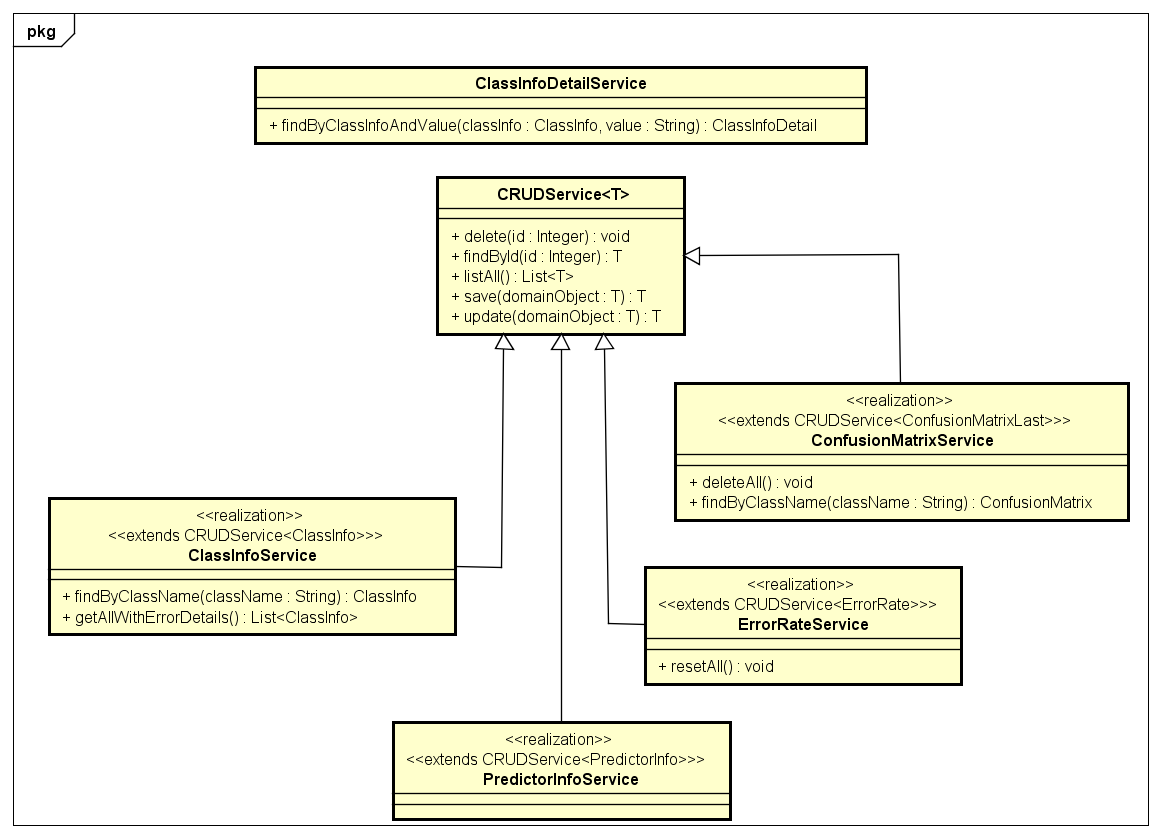
\includegraphics[scale=0.5]{ClassDiagramLengkap/Klasifikasi/Simple_CD_Klasifikasi_Services}
	\caption[Diagram Kelas Modul Kelola Input]{Diagram Kelas Modul Kelola Input}
	\label{fig:Diagram Kelas Modul Kelola Input}
\end{figure}

\subsubsection{\textit{Model}}
\begin{figure}[H]
	\centering
	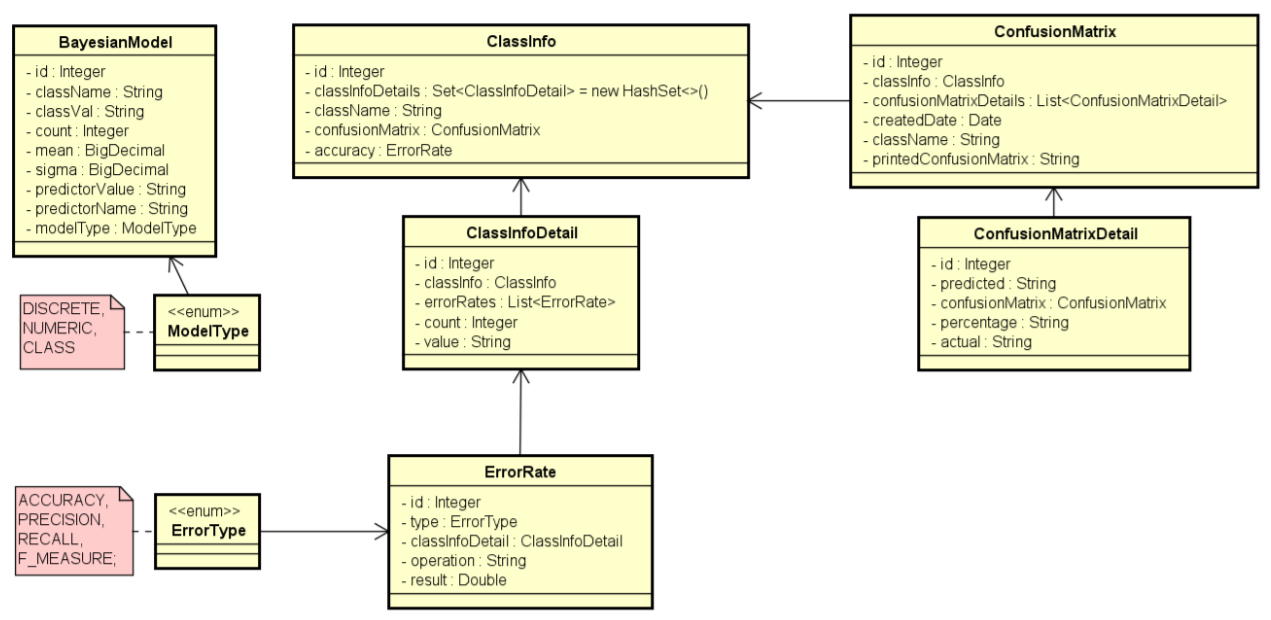
\includegraphics[scale=0.5]{ClassDiagramLengkap/Klasifikasi/Simple_CD_Klasifikasi_Model}
	\caption[Diagram Kelas Modul Kelola Input]{Diagram Kelas Modul Kelola Input}
	\label{fig:Diagram Kelas Modul Kelola Input}
\end{figure}